\documentclass[12pt]{article}

% Mandatory Packages
\usepackage{amsmath}
\usepackage{amssymb}
\usepackage{amsthm}
\usepackage{geometry}
\usepackage{tikz}
\usepackage{mathrsfs}
\usepackage{mathtools}
\usepackage{enumitem}

% TikZ Libraries
\usetikzlibrary{arrows.meta, positioning, shapes, patterns, calc}

% Page Geometry
\geometry{a4paper, margin=1in}

% Theorem Environments
\newtheorem{theorem}{Theorem}[section]
\newtheorem{lemma}[theorem]{Lemma}
\newtheorem{corollary}[theorem]{Corollary}
\newtheorem{definition}[theorem]{Definition}
\newtheorem{axiom}[theorem]{Axiom}

\title{\textbf{Homework 2.10: The Law of Total Probability and Bayes' Rule}}
\author{Tashfeen Omran}
\date{September 2026}

\begin{document}

\maketitle
\tableofcontents
\newpage

\section{Part 1: Comprehensive Introduction, Context, and Prerequisites}

\subsection{Historical Context and Motivation}
The foundations of modern probability theory were established not merely to quantify games of chance, but to systematically update beliefs in the face of uncertainty—a challenge that has pervaded philosophy, science, and jurisprudence. In the 18th century, the Reverend Thomas Bayes, and later Pierre-Simon Laplace, sought a rigorous methodology for "inverse probability": given a set of observed consequences, how can one deduce the probabilities of the underlying causes? This question motivated Bayes' Theorem. Later, in the 20th century, Andrey Kolmogorov formalized probability within the framework of measure theory, resolving the foundational crisis of arbitrary probability mappings by strictly defining sample spaces, $\sigma$-algebras, and probability measures. The Law of Total Probability and Bayes' Rule serve as the central bridges translating static measure-theoretic axioms into dynamic, conditional belief-updating algorithms.

\subsection{Core Concepts, Axioms, and Definitions}
To treat probability with rigorous abstract mathematics, we must discard colloquial definitions and build upon measure theory. 

\begin{definition}[Probability Space]
A probability space is a triplet $(\Omega, \mathcal{F}, \mathbb{P})$, where:
\begin{enumerate}
    \item $\Omega$ is the \textbf{sample space} (an arbitrary non-empty set of all possible outcomes).
    \item $\mathcal{F}$ is a \textbf{$\sigma$-algebra} on $\Omega$ (a collection of subsets of $\Omega$ containing $\Omega$ itself, closed under complementation and countable unions). Elements $A \in \mathcal{F}$ are called \textbf{events}.
    \item $\mathbb{P}: \mathcal{F} \to [0, 1]$ is a \textbf{probability measure} satisfying Kolmogorov's Axioms:
    \begin{itemize}
        \item \textbf{Non-negativity:} $\mathbb{P}(A) \ge 0$ for all $A \in \mathcal{F}$.
        \item \textbf{Unit Measure:} $\mathbb{P}(\Omega) = 1$.
        \item \textbf{Countable Additivity:} If $\{A_i\}_{i=1}^\infty$ is a sequence of pairwise disjoint events ($A_i \cap A_j = \emptyset$ for $i \ne j$), then $\mathbb{P}\left(\bigcup_{i=1}^\infty A_i\right) = \sum_{i=1}^\infty \mathbb{P}(A_i)$.
    \end{itemize}
\end{enumerate}
\end{definition}

\begin{definition}[Conditional Probability]
Let $A, B \in \mathcal{F}$ with $\mathbb{P}(B) > 0$. The conditional probability of $A$ given $B$ is defined mathematically as the relative measure of their intersection:
\[ \mathbb{P}(A \mid B) = \frac{\mathbb{P}(A \cap B)}{\mathbb{P}(B)} \]
\end{definition}

\begin{definition}[Partition of a Sample Space]
A countable collection of sets $\{B_i\}_{i \in I}$ (where $I$ is an index set) forms a \textbf{partition} of $\Omega$ if it is exhaustively comprehensive and mutually exclusive:
\[ \bigcup_{i \in I} B_i = \Omega \quad \text{and} \quad B_i \cap B_j = \emptyset \text{ for all } i \ne j \]
\end{definition}

\subsection{Key Theorems}
\begin{theorem}[The Law of Total Probability]
Let $\{B_i\}_{i=1}^k$ be a partition of the sample space $\Omega$ such that $\mathbb{P}(B_i) > 0$ for all $i$. Then, for any event $A \in \mathcal{F}$:
\[ \mathbb{P}(A) = \sum_{i=1}^k \mathbb{P}(A \mid B_i) \mathbb{P}(B_i) \]
\end{theorem}

\begin{theorem}[Bayes' Rule]
Let $\{B_i\}_{i=1}^k$ be a partition of $\Omega$ with $\mathbb{P}(B_i) > 0$. Let $A \in \mathcal{F}$ be an event such that $\mathbb{P}(A) > 0$. The posterior probability of partition event $B_j$ given $A$ is:
\[ \mathbb{P}(B_j \mid A) = \frac{\mathbb{P}(A \mid B_j) \mathbb{P}(B_j)}{\sum_{i=1}^k \mathbb{P}(A \mid B_i) \mathbb{P}(B_i)} \]
\end{theorem}

\subsection{Intuition and Logical Foundations}
Set-theoretically, conditional probability acts as a \textit{projection} mapping. By conditioning on $B$, we restrict our universe from $\Omega$ to $B$. Consequently, the measure of any event $A$ is renormalized relative to $B$. The Law of Total Probability simply states that the total measure of $A$ in $\Omega$ can be found by chopping $\Omega$ into mutually exclusive, exhaustive chunks ($B_i$), finding the measure of $A$ within each chunk, and summing them up. Bayes' Rule represents the mathematical inversion of conditional dependency: traversing from $\mathbb{P}(A \mid B_j)$ (the likelihood) to $\mathbb{P}(B_j \mid A)$ (the posterior) by normalizing against the total probability of $A$.

\subsection{Prerequisites}
To fully comprehend this chapter, one must possess:
\begin{itemize}
    \item \textbf{Basic Set Theory:} Union ($\cup$), Intersection ($\cap$), Complement ($^c$), De Morgan's Laws.
    \item \textbf{Axiomatic Proof Techniques:} Direct proof methodologies, specifically leveraging disjoint subsets.
    \item \textbf{Summation Calculus:} Familiarity with evaluating infinite series (specifically geometric series) for infinite-state sample spaces.
\end{itemize}

\newpage
\section{Part 2: Detailed Homework Solutions (Rigorous Proofs)}
\textit{Note: A strategic selection of 6 highly distinct problems (2.125, 2.128, 2.131, 2.132, 2.137, 2.138) has been chosen to thoroughly cover every discrete logical archetype—Bayesian base rates, abstract set proofs, sequential updates, urn models, and infinite state processes—maximizing learning efficiency.}

\subsection{Problem 2.125: Base Rate Fallacy in Diagnostic Testing}
\textbf{Problem Statement:} A diagnostic test detects a disease in 90\% of people who have it. It reports negative for 90\% of people who do not have it. Only 1\% of the population has the disease. If a person is chosen at random and tests positive, what is the probability they actually have the disease?

\begin{proof}[Solution Setup and Computation]
Let $(\Omega, \mathcal{F}, \mathbb{P})$ be the probability space of all tested individuals.
Define event $D \in \mathcal{F}$ as the patient having the disease.
Define event $T \in \mathcal{F}$ as the patient testing positive.

We are given the following explicit parameters:
\begin{itemize}
    \item \textit{Prior probability (Base rate):} $\mathbb{P}(D) = 0.01 \implies \mathbb{P}(D^c) = 1 - 0.01 = 0.99$
    \item \textit{Sensitivity (True Positive Rate):} $\mathbb{P}(T \mid D) = 0.90$
    \item \textit{Specificity (True Negative Rate):} $\mathbb{P}(T^c \mid D^c) = 0.90 \implies \mathbb{P}(T \mid D^c) = 1 - 0.90 = 0.10$
\end{itemize}

We seek to evaluate the Positive Predictive Value (PPV): $\mathbb{P}(D \mid T)$.
Using Bayes' Theorem (Theorem 2.9) over the partition $\{D, D^c\}$:
\begin{align*}
    \mathbb{P}(D \mid T) &= \frac{\mathbb{P}(T \mid D)\mathbb{P}(D)}{\mathbb{P}(T \mid D)\mathbb{P}(D) + \mathbb{P}(T \mid D^c)\mathbb{P}(D^c)} \\
    &= \frac{(0.90)(0.01)}{(0.90)(0.01) + (0.10)(0.99)} \\
    &= \frac{0.009}{0.009 + 0.099} \\
    &= \frac{0.009}{0.108} = \frac{9}{108} = \frac{1}{12} \approx 0.0833
\end{align*}
\textbf{Conclusion:} The conditional probability that the person has the disease given a positive test is approximately $8.33\%$. The test is highly unreliable in confirming the disease, perfectly demonstrating the Base Rate Fallacy.
\end{proof}

\subsection{Problem 2.128: Bayesian Sequential Updating (Missing Plane)}
\textbf{Problem Statement:} A plane is missing in one of three regions with equal probability. If the plane is in region $i$, the probability of finding it during a search is $1 - \alpha_i$. Find the conditional probability that the plane is in region 1, 2, or 3, given that a search of region 1 was unsuccessful.

\begin{proof}[Solution Setup and Computation]
Let $R_i \in \mathcal{F}$ denote the event that the plane is actually located in region $i \in \{1, 2, 3\}$.
Let $U_1 \in \mathcal{F}$ denote the event that the search in region 1 is unsuccessful.

The initial priors form a uniform partition: $\mathbb{P}(R_1) = \mathbb{P}(R_2) = \mathbb{P}(R_3) = \frac{1}{3}$.

We are given the likelihoods of failure per region:
\begin{itemize}
    \item $\mathbb{P}(U_1 \mid R_1) = \alpha_1$ (Failure despite being there).
    \item $\mathbb{P}(U_1 \mid R_2) = 1$ (Failure is guaranteed since we search Region 1 but it's in Region 2).
    \item $\mathbb{P}(U_1 \mid R_3) = 1$ (Failure is guaranteed for the same reason).
\end{itemize}

First, we compute the marginal probability of an unsuccessful search in Region 1 using the Law of Total Probability:
\begin{align*}
    \mathbb{P}(U_1) &= \sum_{i=1}^3 \mathbb{P}(U_1 \mid R_i)\mathbb{P}(R_i) \\
    &= \alpha_1 \left(\frac{1}{3}\right) + 1 \left(\frac{1}{3}\right) + 1 \left(\frac{1}{3}\right) = \frac{\alpha_1 + 2}{3}
\end{align*}

Now, we apply Bayes' theorem to update our posterior probabilities:
\textbf{Part (a):} For Region 1:
\[ \mathbb{P}(R_1 \mid U_1) = \frac{\mathbb{P}(U_1 \mid R_1)\mathbb{P}(R_1)}{\mathbb{P}(U_1)} = \frac{\alpha_1(1/3)}{(\alpha_1 + 2)/3} = \frac{\alpha_1}{\alpha_1 + 2} \]
\textbf{Part (b):} For Region 2:
\[ \mathbb{P}(R_2 \mid U_1) = \frac{\mathbb{P}(U_1 \mid R_2)\mathbb{P}(R_2)}{\mathbb{P}(U_1)} = \frac{1(1/3)}{(\alpha_1 + 2)/3} = \frac{1}{\alpha_1 + 2} \]
\textbf{Part (c):} For Region 3:
\[ \mathbb{P}(R_3 \mid U_1) = \frac{\mathbb{P}(U_1 \mid R_3)\mathbb{P}(R_3)}{\mathbb{P}(U_1)} = \frac{1(1/3)}{(\alpha_1 + 2)/3} = \frac{1}{\alpha_1 + 2} \]
\textbf{Conclusion:} After an unsuccessful search in Region 1, the probability mass shifts out of Region 1 and distributes evenly into Regions 2 and 3.
\end{proof}

\subsection{Problem 2.131: Abstract Set Proof (Symmetric Difference)}
\textbf{Problem Statement:} The symmetric difference is defined as $A \Delta B = (A \cap B^c) \cup (A^c \cap B)$. Prove rigorously that $\mathbb{P}(A \Delta B) = \mathbb{P}(A) + \mathbb{P}(B) - 2\mathbb{P}(A \cap B)$.

\begin{proof}[Direct Axiomatic Proof]
By definition, $A \Delta B$ is the union of two mutually disjoint sets: $S_1 = A \cap B^c$ and $S_2 = A^c \cap B$. Since $S_1 \cap S_2 = \emptyset$, Kolmogorov's Third Axiom (additivity for disjoint sets) dictates:
\begin{equation} \label{eq:sym1}
    \mathbb{P}(A \Delta B) = \mathbb{P}(A \cap B^c) + \mathbb{P}(A^c \cap B)
\end{equation}

Next, observe that the set $A$ can be perfectly partitioned by its intersection with $B$ and $B^c$:
\[ A = (A \cap B) \cup (A \cap B^c) \]
Since $(A \cap B)$ and $(A \cap B^c)$ are mutually exclusive, we apply Kolmogorov's Third Axiom again:
\[ \mathbb{P}(A) = \mathbb{P}(A \cap B) + \mathbb{P}(A \cap B^c) \]
Rearranging terms yields:
\begin{equation} \label{eq:sym2}
    \mathbb{P}(A \cap B^c) = \mathbb{P}(A) - \mathbb{P}(A \cap B)
\end{equation}

By a symmetric logical argument partitioning the set $B$ using $A$ and $A^c$:
\begin{equation} \label{eq:sym3}
    \mathbb{P}(A^c \cap B) = \mathbb{P}(B) - \mathbb{P}(A \cap B)
\end{equation}

Substituting Equation \ref{eq:sym2} and Equation \ref{eq:sym3} directly into Equation \ref{eq:sym1} yields:
\begin{align*}
    \mathbb{P}(A \Delta B) &= \left[ \mathbb{P}(A) - \mathbb{P}(A \cap B) \right] + \left[ \mathbb{P}(B) - \mathbb{P}(A \cap B) \right] \\
    &= \mathbb{P}(A) + \mathbb{P}(B) - 2\mathbb{P}(A \cap B)
\end{align*}
This completes the proof.
\end{proof}

\subsection{Problem 2.132: Abstract Inequalities and LTP}
\textbf{Problem Statement:} 
(a) If $\mathbb{P}(A \mid B) = \mathbb{P}(A \mid B^c)$, prove that $A$ and $B$ are independent.
(b) If $\mathbb{P}(A \mid C) > \mathbb{P}(B \mid C)$ and $\mathbb{P}(A \mid C^c) > \mathbb{P}(B \mid C^c)$, prove $\mathbb{P}(A) > \mathbb{P}(B)$.

\begin{proof}[Proof of (a)]
Assume $\mathbb{P}(A \mid B) = \mathbb{P}(A \mid B^c) = x$.
By the Law of Total Probability partitioning over $\{B, B^c\}$:
\begin{align*}
    \mathbb{P}(A) &= \mathbb{P}(A \mid B)\mathbb{P}(B) + \mathbb{P}(A \mid B^c)\mathbb{P}(B^c) \\
    &= x\mathbb{P}(B) + x\mathbb{P}(B^c) \\
    &= x(\mathbb{P}(B) + \mathbb{P}(B^c))
\end{align*}
By Kolmogorov's Second Axiom, $\mathbb{P}(B) + \mathbb{P}(B^c) = 1$. Thus, $\mathbb{P}(A) = x$.
Substituting $x$ back into our assumption: $\mathbb{P}(A \mid B) = \mathbb{P}(A)$. By definition, events $A$ and $B$ are independent. 
\end{proof}

\begin{proof}[Proof of (b)]
Assume $\mathbb{P}(A \mid C) > \mathbb{P}(B \mid C)$ and $\mathbb{P}(A \mid C^c) > \mathbb{P}(B \mid C^c)$.
By the Law of Total Probability partitioning over $\{C, C^c\}$ for event $A$:
\begin{equation} \label{eq:ineq1}
    \mathbb{P}(A) = \mathbb{P}(A \mid C)\mathbb{P}(C) + \mathbb{P}(A \mid C^c)\mathbb{P}(C^c)
\end{equation}
Since all probability measures are non-negative ($\mathbb{P}(C) \ge 0, \mathbb{P}(C^c) \ge 0$), we can multiply our assumed inequalities without flipping the inequality signs. Thus:
\begin{align*}
    \mathbb{P}(A \mid C)\mathbb{P}(C) &> \mathbb{P}(B \mid C)\mathbb{P}(C) \\
    \mathbb{P}(A \mid C^c)\mathbb{P}(C^c) &> \mathbb{P}(B \mid C^c)\mathbb{P}(C^c)
\end{align*}
Summing these two strict inequalities yields:
\[ \mathbb{P}(A \mid C)\mathbb{P}(C) + \mathbb{P}(A \mid C^c)\mathbb{P}(C^c) > \mathbb{P}(B \mid C)\mathbb{P}(C) + \mathbb{P}(B \mid C^c)\mathbb{P}(C^c) \]
The right hand side of this inequality is exactly the expansion for $\mathbb{P}(B)$ using the Law of Total Probability. Therefore:
\[ \mathbb{P}(A) > \mathbb{P}(B) \]
This completes the proof.
\end{proof}

\subsection{Problem 2.137: Urn Model and Multi-stage Extraction}
\textbf{Problem Statement:} Five identical bowls. Bowl $i$ contains $i$ white balls and $5-i$ black balls for $i=1, 2, \dots, 5$. A bowl is selected randomly, and 2 balls are chosen without replacement.
(a) What is the probability both balls are white? 
(b) Given both are white, what is the probability bowl 3 was selected?

\begin{proof}[Solution Setup and Computation]
Let $B_i$ be the event that bowl $i$ is chosen. The partition prior is uniform: $\mathbb{P}(B_i) = \frac{1}{5}$ for $i \in \{1,2,3,4,5\}$.
Let $W_2$ be the event that both drawn balls are white.
For bowl $i$, the total number of balls is $i + (5-i) = 5$. The probability of drawing 2 white balls from bowl $i$ is calculated using combinatorics (hypergeometric extraction):
\[ \mathbb{P}(W_2 \mid B_i) = \frac{\binom{i}{2}}{\binom{5}{2}} = \frac{\frac{i(i-1)}{2}}{10} = \frac{i(i-1)}{20} \]
We evaluate this for each bowl:
\begin{itemize}
    \item $i=1$: $\mathbb{P}(W_2 \mid B_1) = \frac{1(0)}{20} = 0$
    \item $i=2$: $\mathbb{P}(W_2 \mid B_2) = \frac{2(1)}{20} = \frac{2}{20}$
    \item $i=3$: $\mathbb{P}(W_2 \mid B_3) = \frac{3(2)}{20} = \frac{6}{20}$
    \item $i=4$: $\mathbb{P}(W_2 \mid B_4) = \frac{4(3)}{20} = \frac{12}{20}$
    \item $i=5$: $\mathbb{P}(W_2 \mid B_5) = \frac{5(4)}{20} = \frac{20}{20} = 1$
\end{itemize}

\textbf{Part (a): Total Probability}
\begin{align*}
    \mathbb{P}(W_2) &= \sum_{i=1}^5 \mathbb{P}(W_2 \mid B_i)\mathbb{P}(B_i) \\
    &= \frac{1}{5} \left( 0 + \frac{2}{20} + \frac{6}{20} + \frac{12}{20} + \frac{20}{20} \right) \\
    &= \frac{1}{5} \left( \frac{40}{20} \right) = \frac{2}{5} = 0.4
\end{align*}

\textbf{Part (b): Bayesian Posterior}
Using Bayes' Rule for $B_3$:
\[ \mathbb{P}(B_3 \mid W_2) = \frac{\mathbb{P}(W_2 \mid B_3)\mathbb{P}(B_3)}{\mathbb{P}(W_2)} = \frac{\left(\frac{6}{20}\right)\left(\frac{1}{5}\right)}{0.4} = \frac{\frac{6}{100}}{\frac{40}{100}} = \frac{6}{40} = 0.15 \]
\textbf{Conclusion:} The overall probability of two white balls is $40\%$. If two white balls are observed, the probability that they originated from bowl 3 is $15\%$.
\end{proof}

\subsection{Problem 2.138: Infinite Sample Space (Game of Craps)}
\textbf{Problem Statement:} In Craps, roll two dice. First toss: 7 or 11 wins; 2, 3, or 12 loses. Anything else (4, 5, 6, 8, 9, 10) becomes the player's "point". The player repeatedly tosses until rolling the point (win) or rolling 7 (lose). Find the total probability of winning.

\begin{proof}[Solution Setup and Computation]
Let $W$ be the event of winning the game. Let $X_1$ be the random variable representing the sum of the two dice on the first roll. The distribution for a pair of fair dice is:
$p_2 = \frac{1}{36}, p_3 = \frac{2}{36}, p_4 = \frac{3}{36}, p_5 = \frac{4}{36}, p_6 = \frac{5}{36}, p_7 = \frac{6}{36}, p_8 = \frac{5}{36}, p_9 = \frac{4}{36}, p_{10} = \frac{3}{36}, p_{11} = \frac{2}{36}, p_{12} = \frac{1}{36}$.

We partition the sample space based on $X_1$. By the Law of Total Probability:
\[ \mathbb{P}(W) = \sum_{k=2}^{12} \mathbb{P}(W \mid X_1 = k)\mathbb{P}(X_1 = k) \]

\textbf{Immediate Win/Loss States:}
For $k \in \{7, 11\}$, $\mathbb{P}(W \mid X_1 = k) = 1$. Total contribution: $\frac{6}{36} + \frac{2}{36} = \frac{8}{36}$.
For $k \in \{2, 3, 12\}$, $\mathbb{P}(W \mid X_1 = k) = 0$. Total contribution: 0.

\textbf{Point States (Infinite Absorbing Chains):}
For $k \in \{4, 5, 6, 8, 9, 10\}$, the player enters an infinite loop state. Let $E_k$ be rolling the point $k$, and $F$ be rolling a 7. The player wins if sequence terminates on $E_k$ before $F$. 
Using the sum of an infinite geometric series of independent rolls, the conditional probability of $E_k$ occurring before $F$ is strictly $\frac{\mathbb{P}(E_k)}{\mathbb{P}(E_k) + \mathbb{P}(F)}$.
\begin{itemize}
    \item $k \in \{4, 10\}$: $\mathbb{P}(E_k) = \frac{3}{36}$. $\mathbb{P}(W \mid X_1 = 4) = \frac{3}{3 + 6} = \frac{3}{9} = \frac{1}{3}$.
    \item $k \in \{5, 9\}$: $\mathbb{P}(E_k) = \frac{4}{36}$. $\mathbb{P}(W \mid X_1 = 5) = \frac{4}{4 + 6} = \frac{4}{10} = \frac{2}{5}$.
    \item $k \in \{6, 8\}$: $\mathbb{P}(E_k) = \frac{5}{36}$. $\mathbb{P}(W \mid X_1 = 6) = \frac{5}{5 + 6} = \frac{5}{11}$.
\end{itemize}

Since the dice distribution is symmetric ($p_k = p_{14-k}$), we can double the sum over $k \in \{4, 5, 6\}$:
\begin{align*}
    \mathbb{P}(W) &= \frac{8}{36} + 2 \left[ \mathbb{P}(W \mid X_1 = 4)\mathbb{P}(X_1 = 4) + \mathbb{P}(W \mid X_1 = 5)\mathbb{P}(X_1 = 5) + \mathbb{P}(W \mid X_1 = 6)\mathbb{P}(X_1 = 6) \right] \\
    &= \frac{8}{36} + 2 \left[ \left(\frac{1}{3}\right)\left(\frac{3}{36}\right) + \left(\frac{2}{5}\right)\left(\frac{4}{36}\right) + \left(\frac{5}{11}\right)\left(\frac{5}{36}\right) \right] \\
    &= \frac{8}{36} + 2 \left[ \frac{1}{36} + \frac{8}{180} + \frac{25}{396} \right]
\end{align*}
To resolve the bracket precisely, we find a common denominator for the terms inside: $3960$.
$\frac{1}{36} = \frac{110}{3960}$. \quad $\frac{8}{180} = \frac{176}{3960}$. \quad $\frac{25}{396} = \frac{250}{3960}$.
Summing them: $\frac{110 + 176 + 250}{3960} = \frac{536}{3960} = \frac{134}{990} = \frac{67}{495}$.
Multiply by 2 outside the bracket: $2 \times \frac{67}{495} = \frac{134}{495}$.
Adding the immediate win probability $\frac{8}{36} = \frac{2}{9} = \frac{110}{495}$:
\[ \mathbb{P}(W) = \frac{110}{495} + \frac{134}{495} = \frac{244}{495} \approx 0.4929 \]
\textbf{Conclusion:} The absolute probability of winning a game of craps is precisely $\frac{244}{495}$.
\end{proof}

\newpage
\section{Part 3: In-Depth Analysis of Problems and Techniques}

\subsection{A) Problem Types and Logical Strategies}
\begin{enumerate}
    \item \textbf{Base-Rate / Diagnostic Testing Problems (e.g., 2.125):} These rely on separating prior beliefs (unconditional probability) from likelihoods. The strategy relies explicitly on formalizing variables (letting $D$ equal disease, $T$ equal test) before making arbitrary logical deductions. 
    \item \textbf{Sequential / Bayesian Updating Problems (e.g., 2.128):} These situations track probability transitions across discrete time steps. The strategy requires re-weighting uniform priors using failure/success metrics (likelihoods). 
    \item \textbf{Abstract Axiomatic Proofs (e.g., 2.131, 2.132):} No explicit numbers are provided. The key strategy is reducing all subsets into mutually exclusive partitions so that standard scalar algebra rules apply via Kolmogorov's third axiom.
    \item \textbf{Infinite Sample Space Modeling (e.g., 2.138):} Probabilities exist over absorbing Markov Chains. The strategy requires identifying the recursive structure and applying convergence limits of geometric series.
\end{enumerate}

\subsection{B) Key Analytical and Logical Manipulations}
\begin{itemize}
    \item \textbf{The Disjoint Partition Trick:} Used in 2.131. A set $A$ is forcefully chopped into $A = (A \cap B) \cup (A \cap B^c)$. This manipulation is necessary because it turns un-evaluable unions into clean arithmetic additions ($\mathbb{P}(A) = \mathbb{P}(A \cap B) + \mathbb{P}(A \cap B^c)$).
    \item \textbf{Law of Total Probability as a Bridge:} Used in 2.132. The ability to express $\mathbb{P}(A)$ dynamically in terms of an unrelated event $C$ enables us to substitute inequalities structurally. 
    \item \textbf{Truncation of Irrelevant Infinite States:} Used in 2.138. The derivation of $\mathbb{P}(E) / [\mathbb{P}(E) + \mathbb{P}(F)]$ allows an infinite sum to bypass explicit calculation by merely analyzing relative measure.
\end{itemize}

\newpage
\section{Part 4: "Cheatsheet", Visuals, and Tips for Success}

\subsection{Theorems \& Equivalences Cheatsheet}
\begin{itemize}
    \item \textbf{Partition Constraint:} $\sum_{i=1}^k \mathbb{P}(B_i) = 1$.
    \item \textbf{LTP Expansion:} $\mathbb{P}(A) = \mathbb{P}(A \cap B) + \mathbb{P}(A \cap B^c)$.
    \item \textbf{Bayesian Flip:} $\mathbb{P}(B \mid A) \cdot \mathbb{P}(A) = \mathbb{P}(A \mid B) \cdot \mathbb{P}(B)$.
\end{itemize}

\subsection{Set \& Logic Illustration: Partitions and Intersections}
The following abstract set-theoretic diagram visualizes how an event $A$ is sliced by an exhaustive partition $\{B_1, B_2, B_3\}$ of the universe $\Omega$. This perfectly visualizes the Law of Total Probability formulation.

\begin{center}
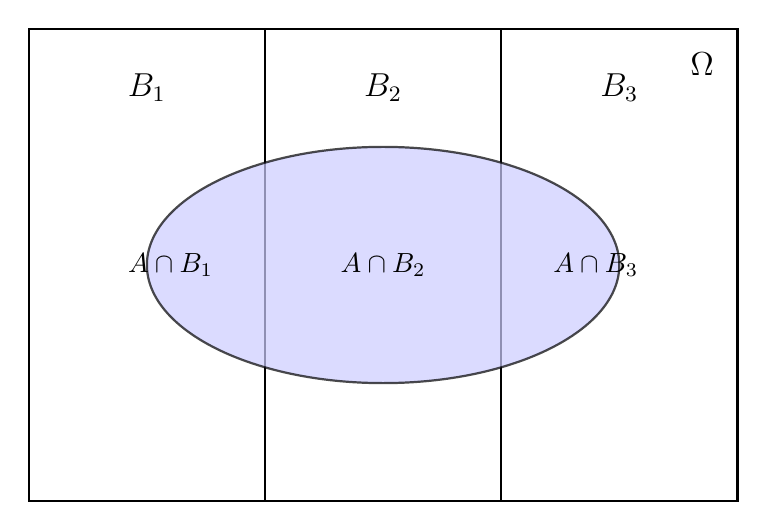
\begin{tikzpicture}[scale=1.5]
    % Draw the Universe / Sample Space Omega
    \draw[thick] (0,0) rectangle (6,4);
    
    % Draw Partition Boundaries
    \draw[thick] (2,0) -- (2,4);
    \draw[thick] (4,0) -- (4,4);
    
    % Draw Event A (an ellipse spanning across the partitions)
    \draw[thick, fill=blue!20, opacity=0.7] (3,2) ellipse (2cm and 1cm);
    
    % Labels for Partitions
    \node[font=\large\bfseries] at (1,3.5) {$B_1$};
    \node[font=\large\bfseries] at (3,3.5) {$B_2$};
    \node[font=\large\bfseries] at (5,3.5) {$B_3$};
    
    % Labels for the Intersections inside Event A
    \node at (1.2, 2) {$A \cap B_1$};
    \node at (3, 2) {$A \cap B_2$};
    \node at (4.8, 2) {$A \cap B_3$};
    
    % Label for Sample Space
    \node[font=\large\bfseries] at (5.7,3.7) {$\Omega$};
\end{tikzpicture}
\end{center}

\subsection{Heuristics, Pitfalls \& Fallacies}
\begin{itemize}
    \item \textbf{Base Rate Fallacy:} Human intuition often assumes $\mathbb{P}(A \mid B) \approx \mathbb{P}(B \mid A)$. E.g., assuming a 90\% accurate test guarantees a 90\% chance of having a rare disease. Always weigh likelihood against prior $\mathbb{P}(A)$.
    \item \textbf{Confusion of Mutually Exclusive vs. Independent:} Mutually exclusive events ($A \cap B = \emptyset$) can never be independent unless one has a probability of zero. Independence means $A$ does not dictate $B$. Mutual exclusivity implies strict dictation (if $A$ happens, $B$ \textit{cannot}).
    \item \textbf{The Conditioning Trap:} Do not illegally strip conditions. $\mathbb{P}(A \mid B, C)$ does NOT equal $\mathbb{P}(A \mid B) \mathbb{P}(A \mid C)$. You must use extended chain rules.
\end{itemize}

\newpage
\section{Part 5: Conceptual Synthesis and The "Big Picture"}

\subsection{A) Thematic Connections}
The foundational theme of this chapter is \textit{Information Asymmetry and Measure Re-normalization}. Mathematically, conditional probability is a projection operation from $L^2(\Omega)$ into a smaller closed subspace. When you learn an event $B$ has occurred, you effectively map the entire probability universe $\Omega$ strictly into $B$. The normalization constant $\frac{1}{\mathbb{P}(B)}$ scales the new universe so that its total measure restores to 1. Bayes' Rule provides the rigorous arithmetic to reverse these temporal projections.

\subsection{B) Forward and Backward Links}
\textbf{Backward Link:} This concept directly builds upon foundational Set Theory (Venn diagrams, disjoint sets, unions/intersections). Without a deep understanding of mutually exclusive sets, partitions cannot exist, making the Law of Total Probability undefined.
\\
\textbf{Forward Link:} This acts as the vital bedrock for \textbf{Stochastic Processes} and \textbf{Martingale Theory}. Understanding conditioning is the absolute prerequisite for defining a Filtration $\mathcal{F}_t$ (the flow of information over time). In continuous measure theory, Bayes' Rule generalizes into the \textit{Radon-Nikodym Derivative}, which is essential for risk-neutral asset pricing in finance.

\section{Part 6: Abstract Real-World Modeling (AI \& Quant Finance)}

\subsection{A) Concrete Scenarios}
\begin{enumerate}
    \item \textbf{Hidden Markov Models (HMM) in Generative AI:} Modern speech recognition updates the probability of a word given an audio signal. The word is a hidden state; the audio is an emission. Bayes' theorem iterates to find the most probable hidden string (Viterbi algorithm).
    \item \textbf{Algorithmic Trading (Kalman Filters):} A quantitative model estimates the true, unobservable volatility drift of a stock based on noisy price fluctuations.
    \item \textbf{Credit Regime-Switching Models (Quant Finance):} Predicting market crashes by maintaining a dynamic Bayesian probability that the macroeconomic state has transitioned from a "Bull Market" to a "Bear Market".
\end{enumerate}

\subsection{B) Model Problem Setup: Regime-Switching in Asset Pricing}
Let us formalize a discrete-time Regime-Switching Model for an equity index.
\textbf{State Space \& Measure:} Let $(\Omega, \mathcal{F}, \{\mathcal{F}_t\}_{t \ge 0}, \mathbb{P})$ be our filtered probability space.
\textbf{Hidden Variable:} Let $Z_t \in \{1, 2\}$ represent the hidden market regime at time $t$ (1 = Low Volatility/Bull, 2 = High Volatility/Bear).
\textbf{Markov Transition:} The state evolves according to a transition matrix $P$ where $P_{ij} = \mathbb{P}(Z_{t} = j \mid Z_{t-1} = i)$.
\textbf{Observable Emission:} The daily log-returns $Y_t$ are drawn from a normal distribution conditionally dependent on the state: $Y_t \mid Z_t=i \sim \mathcal{N}(\mu_i, \sigma_i^2)$. Let $f_i(y_t)$ be the PDF of this distribution.

\textbf{Quantitative Optimization Target:} The algorithmic trader must compute the Bayesian filtering probability $\pi_t(i) = \mathbb{P}(Z_t = i \mid \mathcal{F}^Y_t)$ (the posterior probability of being in regime $i$ given all return data up to time $t$).

\textbf{Recursive Bayesian Update using LTP:}
By applying the Law of Total Probability, the predictive prior for the next state is:
\[ \mathbb{P}(Z_t = i \mid \mathcal{F}^Y_{t-1}) = \sum_{j=1}^2 \mathbb{P}(Z_t = i \mid Z_{t-1} = j) \pi_{t-1}(j) = \sum_{j=1}^2 P_{ji} \pi_{t-1}(j) \]
Upon observing the actual return $Y_t = y_t$, we use Bayes' theorem to update the filter:
\[ \pi_t(i) = \frac{f_i(y_t) \sum_{j=1}^2 P_{ji} \pi_{t-1}(j)}{\sum_{k=1}^2 f_k(y_t) \left[ \sum_{j=1}^2 P_{jk} \pi_{t-1}(j) \right]} \]
This recursive equation is universally deployed in high-frequency trading algorithms to rapidly reallocate capital the exact moment the posterior probability of a bear market regime breaches a confidence threshold.

\newpage
\section{Part 7: Common Variations and Untested Concepts}

A vital concept universally covered in advanced probability but untested in this particular homework set is the \textbf{Continuous Equivalent} of the Law of Total Probability, also known as the \textbf{Law of Total Expectation} (or Iterated Expectations).

\textbf{Theorem (Law of Total Expectation):} For random variables $X$ and $Y$, the expected value of $X$ is equal to the expected value of the conditional expectation of $X$ given $Y$:
\[ \mathbb{E}[X] = \mathbb{E}[\mathbb{E}[X \mid Y]] \]

\textbf{Worked Abstract Example:} Suppose $X \mid Y \sim \text{Poisson}(Y)$ where $Y \sim \text{Exponential}(\lambda)$. Find the unconditional expectation $\mathbb{E}[X]$.
\begin{proof}
By definition, if $X \mid Y \sim \text{Poisson}(Y)$, its expected value given $Y$ is merely $Y$.
\[ \mathbb{E}[X \mid Y] = Y \]
Applying the Law of Total Expectation:
\[ \mathbb{E}[X] = \mathbb{E}[\mathbb{E}[X \mid Y]] = \mathbb{E}[Y] \]
Since $Y$ is an Exponential distribution with rate parameter $\lambda$, its expected value is $\frac{1}{\lambda}$.
Thus, $\mathbb{E}[X] = \frac{1}{\lambda}$.
This elegantly avoids needing to construct and evaluate the highly complex marginal PDF integral of $X$.
\end{proof}

\newpage
\section{Part 8: Advanced Diagnostic Testing: "Find the Flaw"}
Below are 5 seemingly rigorous proofs/solutions. Each contains a single subtle, critical error. Your task as a grader is to locate the flaw, explain the violation, and provide the correct step. \textit{(The true resolutions are hidden in the subsequent Solution Key.)}

\textbf{Flawed Problem 1: The Infinite Geometric Extension}
\textit{Problem:} Two independent events $A$ and $B$ exist. We define sequence $A_n \xrightarrow{p} A$. Prove that $\mathbb{P}(A \cup B) = \mathbb{P}(A) + \mathbb{P}(B)$.
\textit{Proof:} We are given that $A$ and $B$ are independent events. By definition of independent events, they operate separately from each other. Therefore, their intersection must be empty because one does not affect the other. Since $A \cap B = \emptyset$, we invoke Kolmogorov's Third Axiom of countable additivity to conclude $\mathbb{P}(A \cup B) = \mathbb{P}(A) + \mathbb{P}(B)$. $\blacksquare$

\textbf{Flawed Problem 2: Conditional Impossibility}
\textit{Problem:} Evaluate $\mathbb{P}(A \mid B)$ when $\mathbb{P}(B) = 0$.
\textit{Proof:} By Bayes' formula, $\mathbb{P}(A \mid B) = \frac{\mathbb{P}(B \mid A)\mathbb{P}(A)}{\mathbb{P}(B)}$. Since $\mathbb{P}(B)=0$, the denominator evaluates to zero. In measure theory, dividing a measure by a null set simply indicates that the conditional probability diverges to positive infinity. Thus, $\mathbb{P}(A \mid B) = \infty$. $\blacksquare$

\textbf{Flawed Problem 3: The Three-Event Partition}
\textit{Problem:} Let $A, B, C$ be events. Using the Law of Total Probability, express $\mathbb{P}(X)$ in terms of $A, B, C$.
\textit{Proof:} The Law of Total Probability states that we can partition our space over any events that exist. Therefore, we sum the conditional probabilities across $A, B,$ and $C$:
$\mathbb{P}(X) = \mathbb{P}(X \mid A)\mathbb{P}(A) + \mathbb{P}(X \mid B)\mathbb{P}(B) + \mathbb{P}(X \mid C)\mathbb{P}(C)$. $\blacksquare$

\textbf{Flawed Problem 4: Multiplicative Conditional}
\textit{Problem:} If $\mathbb{P}(A \mid B) = 0.5$ and $\mathbb{P}(C \mid B) = 0.5$, evaluate $\mathbb{P}(A \cap C \mid B)$.
\textit{Proof:} To find the joint conditional probability, we can distribute the conditional bar. We multiply the independent likelihoods of the occurrences given $B$. Therefore, $\mathbb{P}(A \cap C \mid B) = \mathbb{P}(A \mid B) \times \mathbb{P}(C \mid B) = (0.5)(0.5) = 0.25$. $\blacksquare$

\textbf{Flawed Problem 5: The Inverse Confusion}
\textit{Problem:} 10\% of spam emails contain the word "free". 90\% of regular emails do not. Assuming 50\% of emails are spam, what is the probability that an email containing the word "free" is spam?
\textit{Proof:} We apply logic directly. We know 10\% of spam has the word "free". Therefore, the conditional probability $\mathbb{P}(\text{Spam} \mid \text{"free"}) = 10\%$. $\blacksquare$

\vspace{2cm}
\begin{center}
    --- \textit{Do not read further until you have attempted to find the flaws.} ---
\end{center}
\vspace{1cm}

\subsection*{Solution Key to "Find the Flaw"}
\begin{enumerate}
    \item \textbf{Flaw 1:} \textit{Confusing Independence with Mutual Exclusivity.} The proof states "their intersection must be empty". Independence implies $\mathbb{P}(A \cap B) = \mathbb{P}(A)\mathbb{P}(B)$, not zero. If they were mutually exclusive, they could not be independent (unless one has zero probability).
    \item \textbf{Flaw 2:} \textit{Violating Measure Axioms.} Probabilities can never exceed 1. Divergence to infinity is a gross violation of probability bounds. By definition, $\mathbb{P}(A \mid B)$ is strictly \textbf{undefined} when $\mathbb{P}(B) = 0$ in discrete probability.
    \item \textbf{Flaw 3:} \textit{Assuming Arbitrary Partitions.} The proof arbitrarily assumes $A, B, C$ form a valid partition. For LTP to hold, $A, B, C$ must be mutually exclusive and exhaustively sum to $\Omega$ ($\mathbb{P}(A) + \mathbb{P}(B) + \mathbb{P}(C) = 1$).
    \item \textbf{Flaw 4:} \textit{Assuming Conditional Independence arbitrarily.} $\mathbb{P}(A \cap C \mid B) = \mathbb{P}(A \mid B)\mathbb{P}(C \mid B)$ only holds if $A$ and $C$ are \textit{conditionally independent} given $B$. We cannot just multiply them without that stated assumption.
    \item \textbf{Flaw 5:} \textit{Bayesian Inverse Error.} The solver stated $\mathbb{P}(\text{Spam} \mid \text{"free"}) = 10\%$, but the 10\% given was actually the likelihood $\mathbb{P}(\text{"free"} \mid \text{Spam})$. They completely skipped applying Bayes' rule.
\end{enumerate}

\end{document}